\section{Introduction}

Neural operators learn maps between function spaces and can amortize expensive numerical simulation across many physical configurations \citep{li2021fno,li2023gino,wu2024transolver}. Recently, transformer-based neural operators have improved the scalability and accuracy of operator learning across diverse PDEs and million-point geometries. They make such large-scale computation possible by compressing irregular meshes into latent tokens, distributing the computation, or decoupling global state estimation from pointwise decoding \citep{alkin2024upt,luo2025transolverpp,zhou2026transolver3}. In engineering applications, however, evaluation efficiency is as important as scalability. Yet how neural operators can flexibly allocate computation at inference remains largely unexplored.

Neural-operator training data are typically generated by numerical solvers on meshes that are uniform or designed for numerical convergence. Learned models are consequently evaluated under the same sampling distribution, which may ignore the strongly localized structure of many PDE solutions. Shocks, boundary layers, contact interfaces, and stress concentrations often occur in localized regions and require finer resolution, whereas smooth regions can be represented with fewer samples. This creates a dilemma: preserving the training distribution wastes samples in smooth regions, while reallocating them to critical regions changes the sampling measure. Can a neural operator reallocate a given sampling budget without changing the operator it represents?


Existing efforts address neighboring capabilities. First, resolution
generalization studies how neural operators extrapolate across grid sizes,
point counts, or compatible discretizations while preserving the underlying
sampling distribution \citep{li2021fno,li2023gino,liu2023nuno,alkin2024upt,
zhou2026transolver3,gao2025discretization}. These methods make resolution
changes feasible, but do not by themselves provide a mechanism for spatially reallocating samples according to local physical or solution structures. Second, adaptive sampling and refinement
methods predict where a numerical mesh or point set should be refined, often
as part of a solver pipeline or through a separately trained refinement model
\citep{huang2021meshgeneration,obiols2023adarnet,rowbottom2024gadaptivity}.
They address spatial allocation, but do not specify how a frozen neural
operator should preserve its target integral when that allocation changes the
sampling measure. Third, test-time compute scaling increases inference effort
through adaptive reasoning or iterative physical prediction
\citep{snell2024scalingllmtesttime,lippe2023pderefiner,jenkins2026atca,
serrano2026splitting}. These works establish the value of allocating additional
computation at inference, but leave open the spatial counterpart: reallocating
input samples for operator evaluation while retaining the same learned map.

We introduce AdaSolver to address this gap. We view spatial sampling density as a controllable inference resource for allocating computation at test time. From a continuous-operator perspective, we characterize how shifts in sampling density introduce sampling bias into Transolver. We develop a sampling-density-consistent Transolver that corrects this bias through self-normalized importance weighting. This measure correction enables adaptive test-time sampling driven by geometry or physics priors, a low-cost coarse prediction, or a cache-aware learned refinement policy that reuses intermediate features. Figure~\ref{fig:adasolver_overview} illustrates the AdaSolver framework and its alternative test-time sampling strategies.
\begin{figure}[h!]
    \centering
    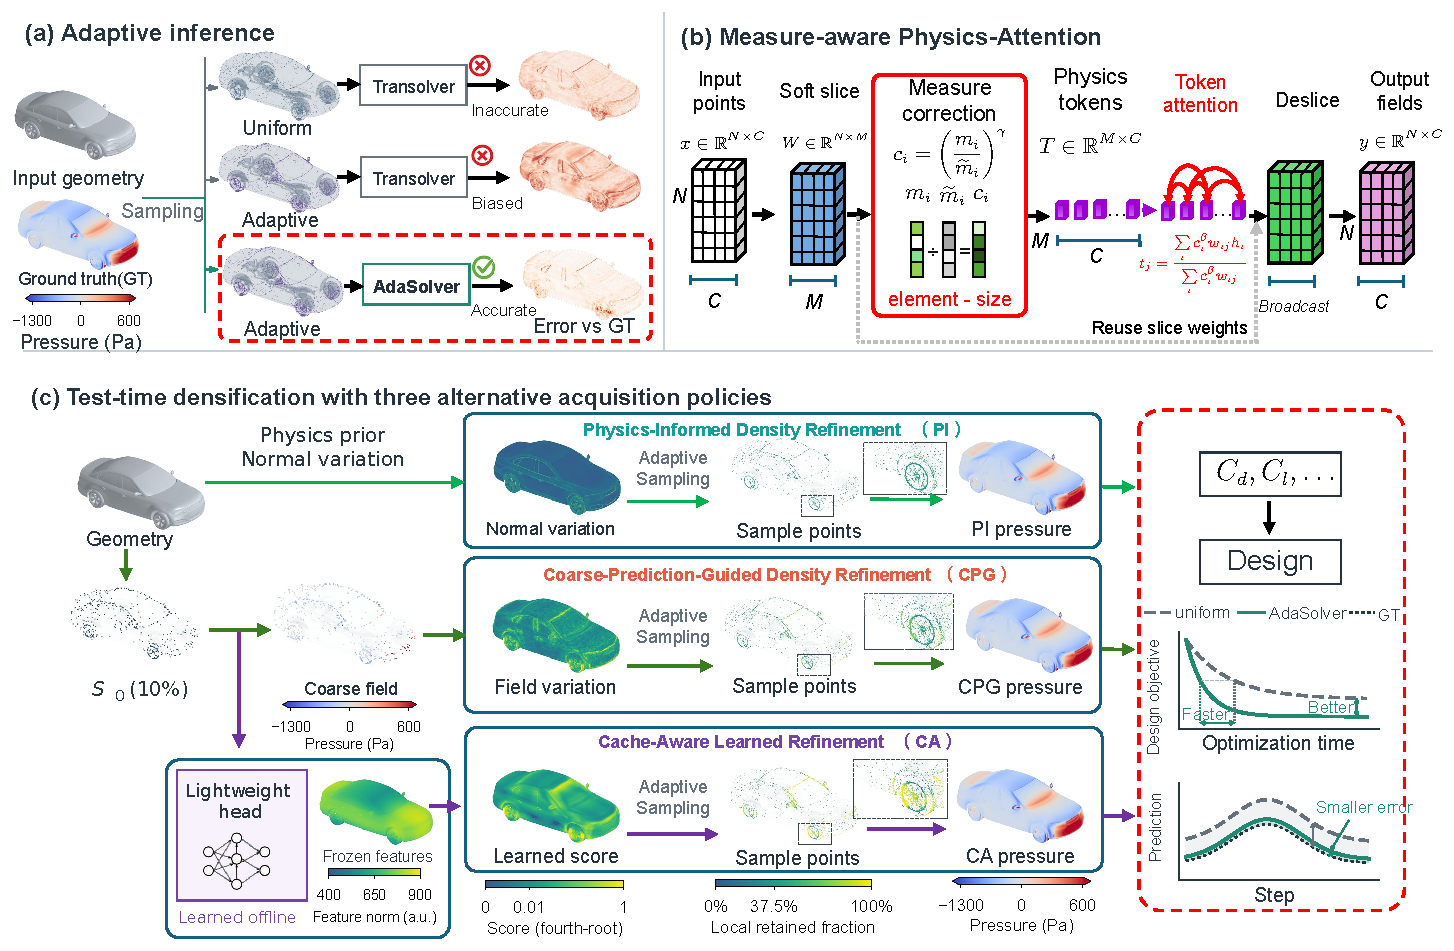
\includegraphics[width=\linewidth]{figures/fig1_overview.pdf}
    \caption{\textbf{AdaSolver overview.}
    (a) Adaptive inference with measure correction.
    (b) Corrected aggregation, token attention, and deslicing.
    (c) Geometry priors, coarse predictions, and a lightweight head on frozen
    features provide alternative refinement signals. The frozen operator evaluates
    the selected points and supplies aerodynamic quantities for design. The
    rightmost curves illustrate the design objectives schematically.}
    \label{fig:adasolver_overview}
\end{figure}


We summarize our contributions as follows: (i) to our knowledge, we provide the first systematic exploration of adaptive spatial sampling as a new axis of test-time scaling for neural operators, revealing sampling-measure shift as a fundamental challenge when reallocating spatial computation at inference; (ii) we introduce AdaSolver, which enables measure-consistent test-time sampling and supports diverse scaling strategies based on physics and geometry priors, coarse predictions, and learned refinement signals; and (iii) we demonstrate consistent improvements in the accuracy--compute trade-off across five standard PDE benchmarks and three industrial aerodynamic tasks, and further show that AdaSolver accelerates surrogate-based airfoil and wing optimization while achieving comparable or improved CFD-validated aerodynamic performance.